% Created 2021-01-30 Sat 13:00
% Intended LaTeX compiler: pdflatex
\documentclass[11pt]{article}
\usepackage[utf8]{inputenc}
\usepackage[T1]{fontenc}
\usepackage{graphicx}
\usepackage{grffile}
\usepackage{longtable}
\usepackage{wrapfig}
\usepackage{rotating}
\usepackage[normalem]{ulem}
\usepackage{amsmath}
\usepackage{textcomp}
\usepackage{amssymb}
\usepackage{capt-of}
\usepackage{hyperref}
\usepackage{amsthm}
\usepackage{url}
\usepackage[margin=.5in]{geometry}
\usepackage{hyperref}
\usepackage[dvipsnames]{xcolor}
\usepackage{booktabs}
\usepackage{enumitem}
\newtheorem*{definition}{Definition}
\newtheorem*{example}{Example}
\newtheorem*{theorem}{Theorem}
\newtheorem*{corollary}{Corollary}
\newtheorem*{exercise}{Exercise}
\newtheorem*{problem}{Problem}
\newtheorem{question}{Question}
\newcommand{\gr}{\textcolor{ForestGreen}}
\newcommand{\rd}{\textcolor{red}}
\newcommand{\R}{\mathbb{R}}
\newcommand{\p}{\mathbb{P}}
\newcommand{\E}{\mathbb{E}}
\newcommand{\frall}{\ \forall}
\newcommand{\st}{_{s_t}}
\newcommand{\var}{\operatorname{Var}}
\newcommand{\cov}{\operatorname{Cov}}
\newcommand{\cor}{\operatorname{Cor}}
\author{Chris Ackerman\thanks{I worked on this problem set with Ekaterina Gurkova, Luna Shen, Ben Pirie and Ali Haider Ismail.}}
\date{\today}
\title{Econ202B HW2}
\hypersetup{
 pdfauthor={Chris Ackerman\thanks{I worked on this problem set with Ekaterina Gurkova, Luna Shen, Ben Pirie and Ali Haider Ismail.}},
 pdftitle={Econ202B HW2},
 pdfkeywords={},
 pdfsubject={},
 pdfcreator={Emacs 28.0.50 (Org mode 9.3)}, 
 pdflang={English}}
\begin{document}

\maketitle
\tableofcontents

\newpage

\section{Question 2}
\label{sec:orgcf89e3e}
  \begin{enumerate}[label=\alph*)]
\item 
\begin{align*}
\intertext{We want to show $\pi (s) = \pi (s) P$.}
P &= \begin{bmatrix}
\rho + (1 - \rho)\pi (s_1) & (1 - \rho)\pi (s_2) & \ldots & (1 - \rho) \pi (s_n)\\
(1 - \rho)\pi (s_1) & \rho + (1 - \rho)\pi(s_2) & \ldots & (1 - \rho)\pi(s_n)\\
\vdots & & \ddots & \vdots \\
(1 - \rho)\pi(s_1) & \ldots & & \rho + (1 - \rho) \pi (s_n)
\end{bmatrix}\\
\intertext{Solving the equation $\pi (I - P) = 0$,}
(1 - \rho) \left\{(1 - \pi(s_j))s_j - \pi (s_j) \sum_{s_i \ne s_j} s_i\right\} &= 0 \ \forall j\\
\frac{s_j}{\pi(s_j)} &= \sum s_j \ \forall j\\
&= 1 \\
\implies s_j &= \pi (s_j)
\end{align*}
\item
\begin{align*}
\cor(X_t, X_{t + 1}) &= \frac{\cov(X_t, X_{t + 1})}{\sqrt{\var(X_t)\var{X_{t + 1}}}}\\
&= \frac{\E[X_t X_{t + 1}] - \E[X_t]^2}{\var{X_t}}\\
\intertext{Define the realized state as $x(s_t)$, where $s_t$ is our Markov chain. Now we want to find an expression for $\E[X_t X_{t + 1}]$.}
\E[X_T X_{t + 1}] &= \E[\E[X_t X_{t + 1}\mid s_t]]\\
&= \sum_i P(s_t = a_i)\E[X_t X_{t + 1} \mid s_t = a_i]\\
&= \sum_i \Pi(a_i)x(a_i)\E[X_{t + 1}\mid x_t = a_i]\\
&= \sum_i \Pi(a_i) x(a_i) \left\{[\rho + (1 - \rho) \Pi(a_i)]x(a_i) + (1 - \rho)\sum_{j \ne i} \Pi(a_i)x(a_j)\right\}\\
&= \sum_i \pi(a_i) x(a_i) \left\{\rho x(a_i) + (1 - \rho) \E[X_t]\right\}\\
&= \sum \rho \pi(a_i)x^2(a_i) + (1- \rho) \pi(a_i) x(a_i) \E[X_t]\\
&= \rho(\var(X_t)) + \E[X_t]^2\\
\implies \cov(X_t X_{t + 1}) &= \rho\\
\intertext{To get $k^{\text{th}}$ order autocorrelation, use the fact that}
\E[X_{t + 1} \mid x_t] &= \rho X_t + (1 - \rho) \E[X_t].\\
\intertext{We're going to perform induction on this equation. Suppose that the $k - 1^{\text{ts}}$ autocorrelation takes the form}
\E[X_{t + k} \mid X_{t + 1}] &= \rho^{k - 1} X_{t + 1} + (1 - \rho^{k - 1})\E[X_{t + 1}]\\
\implies \E[X_{t + k} \mid X_t] &= \E[E[X_{t + k} \mid X_{t + 1}]\mid X_t]\\
&= \rho^k X_t + (1 - k) \E [X_t].\\
\intertext{This is the same term we got earlier, but now we have $\rho^k$ instead of $\rho$.}
\end{align*}
\end{enumerate}
\newpage

\section{Question 3}
\label{sec:org4e86124}

Bellman Equations:
\begin{align*}
V_U(s_t) &= z + \beta \left\{\theta\st q(\theta\st)\E\st [V_E(s')] + (1 - \theta\st q (\theta\st)) \E\st [V_U(s')]\right\}\\
V_E(s_t) &= w(s_t) + \beta \left\{(1 - \delta) \E\st [V_E(s')] + \delta \E\st [V_u(s')]\right\}\\
\Pi_V(s_t) &= -c + \beta \left\{ q(\theta\st)\E\st [\Pi_F(s')] + (1 - q(\theta\st)) \E\st[\Pi_V (s')]\right\}\\
\Pi_F(s_t) &= y(s_t) - w(s_t) + \beta \left\{ (1 - \delta) \E\st [\Pi_F(s')]+ (1 - q(\theta\st)) \E\st[\Pi_V (s')]\right\}
\end{align*}

Surplus Equation:
\begin{align*}
\Sigma(s_t) &= \Pi_F - \Pi_V + V_E - V_U\\
\Pi_V &= 0\tag{free entry}\\
\implies \Sigma(s_t)
&=
y(s_t) - w(s_t) + \beta \left\{ (1 - \delta) \E\st [\Pi_F(s')]+ (1 - q(\theta\st)) \E\st[\Pi_V (s')]\right\}\\
&\ +w(s_t) + \beta \left\{(1 - \delta) \E\st [V_E(s')] + \delta \E\st [V_u(s')]\right\}\\
&\ - z + \beta \left\{\theta\st q(\theta\st)\E\st [V_E(s')] + (1 - \theta\st q (\theta\st)) \E\st [V_U(s')]\right\}\\
&= y(s_t) -z + \beta\left\{1 - \delta - \phi \theta\st q(\theta\st)\E\st[\Sigma(s')]\right\}
\end{align*}

Free entry:
\begin{align*}
\Pi_V(s_t) &= -c + \beta \left\{ q(\theta\st)\E\st [\Pi_F(s')] + (1 - q(\theta\st)) \E\st[\Pi_V (s')]\right\}\\
&=0 \\
\implies c &=\beta \left\{ q(\theta\st)\E\st [\Pi_F(s')] + (1 - q(\theta\st)) \E\st[\Pi_V (s')]\right\}\\
&= \beta (1 - \phi) q(\theta\st)\E\st[\Sigma(s')] + \underbrace{\beta \E\st [\Pi_V(s')]}_0\\
&= \beta (1 - \phi) q(\theta\st)\E\st[\Sigma(s')]
\end{align*}
\newpage

\section{Question 4}
\label{sec:org27e8c00}
  \begin{enumerate}[label=\alph*)]
\item
  \begin{align*}
c &= \beta (1 - \phi) (q(\theta) + q'(\theta) h \Delta \theta (s))(\Sigma + h \E [\Delta \Sigma (s') \mid s])\\
&= \beta (1 - \phi) (q(\theta) \Sigma + hq'(\theta)\Delta \theta (s) \Sigma + \rd{\underbrace{h^2 q'(\theta) \Delta \theta(s) \E[\Delta \Sigma (s') \mid s]}_{\approx 0}} + hq(\theta) \E [\Delta \Sigma (s') \mid s])\\
&= \beta (1 - \phi) (q(\theta)\Sigma + h\gr{\left\{q'(\theta) \Delta \theta (s) \Sigma + q(\theta) \E[\Delta  \Sigma (s') \mid s]\right\}})\\
c &= \beta (1 - \phi) q(\theta)\Sigma \tag{1}\\
0 &= \beta (1- \phi) \{q'(\theta) \Delta \theta (s) \Sigma + q(\theta) \E [\Delta \Sigma (s') \mid s]\}\tag{2}\\
\Sigma (s) + h \Sigma (s) &= y + h \Delta y(s) - z + \beta [1 - \delta - \phi (\theta + h\Delta (s))(q(\theta) + q'(\theta) h \Delta \theta (s)))](\Sigma + h \E[\Delta \Sigma (s')\mid s])\\
\intertext{Some algebra \ldots}
\implies \Sigma &= y - z + \beta (1 - \delta - \phi \theta q(\theta))\Sigma\tag{3}\\
\Delta \Sigma (s) &= \Delta y(s) + \beta \{\phi \Sigma \Delta \theta (s) (\theta q(\theta))' + (1 - \delta - \phi \theta q(\theta)) \E [\Delta \Sigma (s') \mid s]\}\tag{4}
  \end{align*}
\item
\begin{align*}
0 &= \beta (1- \phi) \{q'(\theta) \Delta \theta (s) \Sigma + q(\theta) \E [\Delta \Sigma (s') \mid s]\}\\
\E[0] &= \E[\beta (1- \phi) \{q'(\theta) \Delta \theta (s) \Sigma + q(\theta) \E [\Delta \Sigma (s') \mid s]\}]\\
&= \beta (1 - \phi) \{q'(\theta) \Delta \Sigma \E[\theta (s)] + q(\theta) \E[\E[\Delta \Sigma (s') \mid s]].
\end{align*}
Since none of the parameters here should be zero, this equation only holds when $\E[\Delta \theta (s)] = \E [\Delta \Sigma (s)] = 0$.
\item
\begin{align*}
\intertext{Starting with a few relationships \ldots}
\frac{dq}{d\theta} &= q'(\theta)\\
\frac{1}{\alpha} &= -\frac{q}{\theta q'(\theta)}\\
\E[\Delta \Sigma (s') \mid s] &= \rho \Delta (s) + (1 - \rho)\E[\Delta \Sigma (s')]\\
&= \rho \Delta \Sigma (s)\\
\intertext{Going back to the free entry condition, }
q'(\theta) \Delta \theta (s) \Sigma &= - q (\theta) \rho \Delta \Sigma (s)\\
\frac{\Delta \theta (s)}{\theta} &= - \frac{q(\theta)}{q'(\theta) \theta} \rho \frac{\Delta \Sigma (s)}{\Sigma}\\
&= \frac{\rho}{\alpha} \frac{\Delta \Sigma (s)}{\Sigma}.
\end{align*}
This relationship says that the elasticity of tightness to surplus is the ratio of the autocorrelation term with the elasticity of tightness to the vacancy filling rate. Intuitively, vacancy filling increases as the surplus increases (since each worker/filled vacancy produces more output), and this effect is larger when $\rho$ is larger (since the large surplus is expected to persist in future periods).
\item
\begin{align*}
\intertext{Starting from the equation for changes in surplus,}
\Delta \Sigma(s) &= \Delta y(s) + \beta \left\{\phi \Sigma \theta (s) (\theta q (\theta))' + (1 - \delta - \phi \theta q(\theta))\E[\Delta \Sigma (s') \mid s]\right\}\\
&= \Delta y(s) + \beta \left\{\phi (\theta q (\theta))' \theta \frac{\rho}{\alpha} \Delta \Sigma (s) + (1 - \delta - \phi \theta q(\theta)) \rho \Sigma (s)\right\}\\
&= \Delta y(s) + \beta \left\{\phi (1 - \alpha) \theta q(\theta) \frac{\rho}{\alpha} \Sigma (s) + (1 - \delta - \phi \theta q (\theta))\rho \Delta \Sigma(s)\right\}\\
&= \frac{\Delta y(s)}{1 - \beta \rho\{1 - \delta - \phi \theta q(\theta)/\alpha\}}\\
\intertext{Using the closed form for the surplus equation, we get}
\frac{\Delta \Sigma (s)}{\Sigma} &= \frac{\Delta y(s)}{y} \frac{y/z}{y/z - 1} \frac{1 - \beta (1 - \delta - \phi \theta q (\theta))}{1 - \beta \rho \{1 - \delta - \phi \theta q(\theta) / \alpha\}}
\end{align*}
\end{enumerate}

\newpage
\section{Question 5}
\label{sec:org746bf03}
\begin{table}[htp]
\begin{center}
\begin{tabular}{rcc}
Variable & Expression & Value\\
\toprule
$\theta q(\theta)$ & &$0.45$  \\
$\delta $ && $0.034$  \\
$\frac{y}{z}$ & &$2.5$  \\
$\phi$ & $-\frac{\theta}{q} \frac{dq}{d \theta}$& $0.72$ \\
$\rho$ & $0.878^{1/3}$ & $0.957$ \\
$\beta$ & $0.953^{1/12}$ & $0.995$ 
\end{tabular}
\end{center}
\end{table}

\newpage

\section{Question 6}
\label{sec:orgbe874ac}
\begin{figure}[htp]
\begin{center}
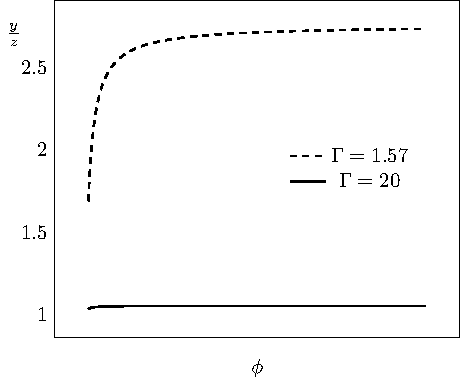
\includegraphics[width=.5\textwidth, keepaspectratio=true]{yz_plot.pdf}
\end{center}
\end{figure}
Hagedorn and Manovskii criticize approaches that impose the Hosios condition because it fails to accurately match elasticities we see in the data. Instead, they proceed by matching the elasticity directly  and choosing parameters that accomodate this value. As such, they're able to calibrate a model that matches observed elasticity more closely, whereas Shimer was off by a factor of 20.
\end{document}